%!TEX root = ../thesis.tex
\define{\chapterpath}{appendix}
\define{\imgpath}{appendix/img}

\define{\twoplanningwidth}{0.7}
\define{\threeplanningwidth}{1}

%%
\chapter{Appendix}
\label{appendix}

\section{Additional visuals of uncertainty}
\label{appendix:uncertaintymeaning}

This section present the illustration of the planning method relying on sampling teaching signal and  asking every hypothesis if each of those signals are expected or not for the given state-action pair. 

We present the case where the models between hypothesis are identical. As depicted in Figure~\ref{fig:uncertaintymeaningupdownexpectedright}, when selecting action down in state 3 and if the user sends a signal in the right part of the feature space, both hypothesis agree that this particular signal is unexpected given this state-action pair. Hypothesis 1 expects a signal of meaning ``incorrect'', and the teacher signal is classified as being of class ``correct''. Hypothesis 2 expects a signal of meaning ``incorrect'' and the teacher signal is classified as being of class ``correct''. Therefore receiving this particular signal after taking action down in state 3 has low uncertainty.

\begin{figure}[!ht]
  \centering
  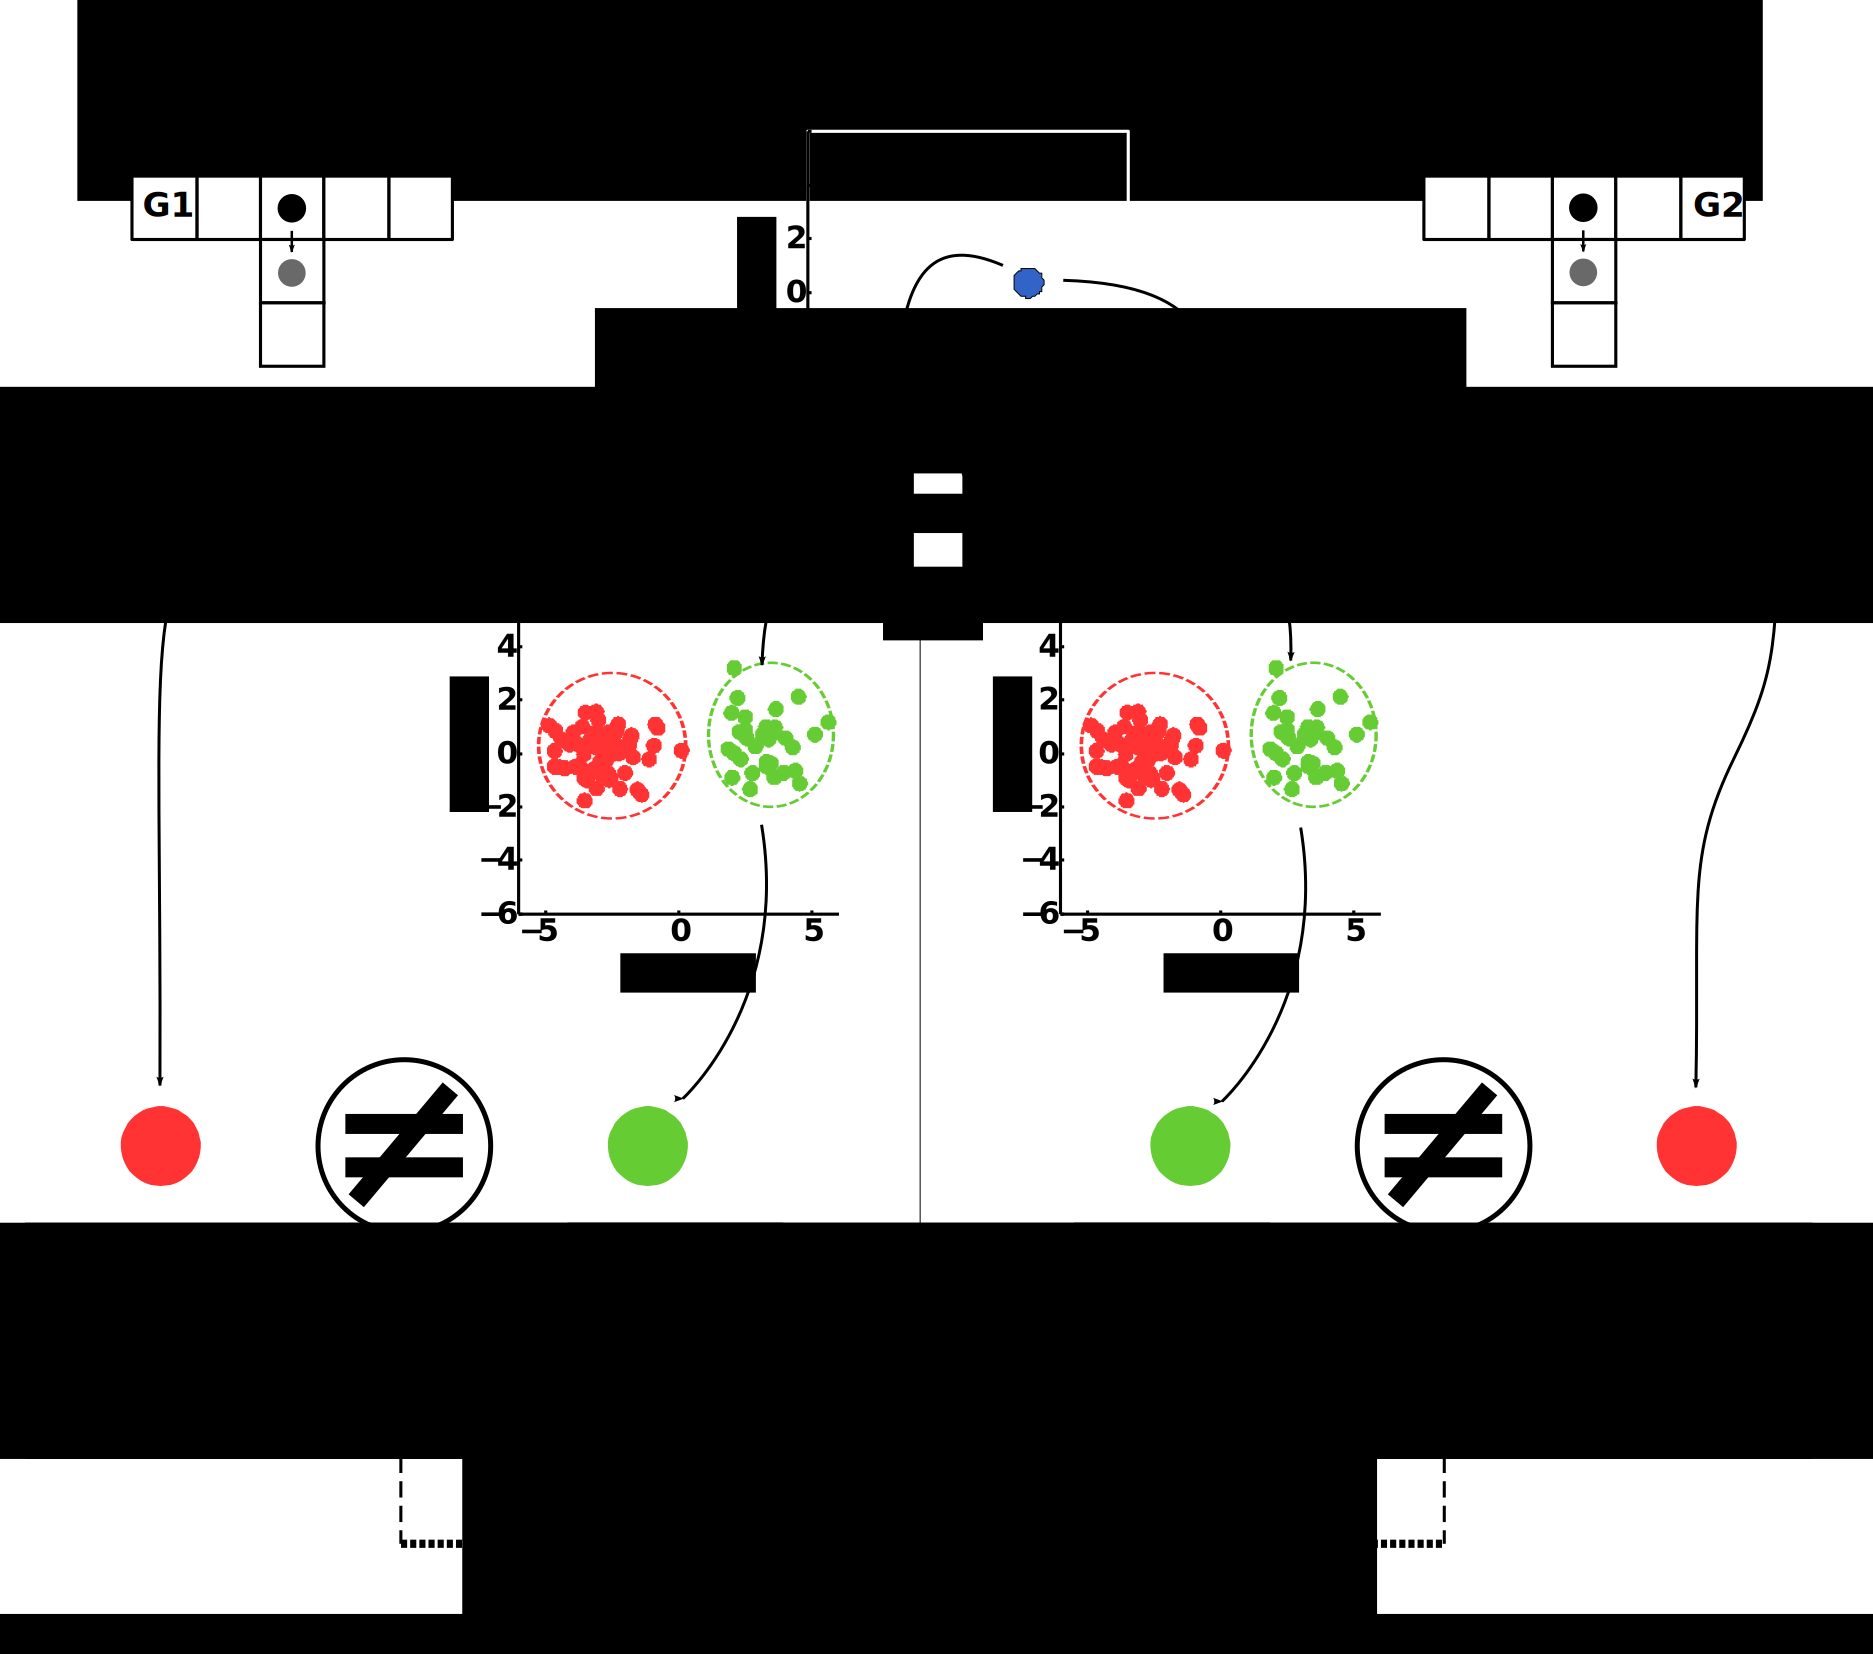
\includegraphics[width=\threeplanningwidth\columnwidth]{\visualspdf/planning/planning_up_down_expected_unmatched.pdf}
  \caption{Matching between expected labels and the prediction of a teaching signal sample on the right side of the feature space for the two hypothesis if the agent performs action down in state 3 and the two hypothesis currently have a symmetric interpretation of signals from Figure~\ref{fig:planningupdown}. Both hypothesis agree that the label associated to a signal on the right side of the feature space does not match with the label predicted given the frame and the state-action pair considered. Therefore there is no uncertainty associated to this state-action pair and the agent should not select action down in order to disambiguate between hypothesis.}
  \label{fig:uncertaintymeaningupdownexpectedright}
\end{figure}

This same process can be executed for any teaching signal. For example, as depicted in Figure~\ref{fig:uncertaintymeaningupdownexpectedleft}, considering a teaching signal on the left side of the feature space, if the agent performs action down in state 3, both hypothesis agree that this particular signal is expected. Hypothesis 1 expects a signal of meaning ``incorrect'', and the teacher signal is classified as being of class ``incorrect''. Hypothesis 2 expects a signal of meaning ``incorrect'' and the teacher signal is classified as being of class ``incorrect''. Therefore receiving this particular signal after taking action down in state 3 has low uncertainty.

\begin{figure}[!ht]
  \centering
  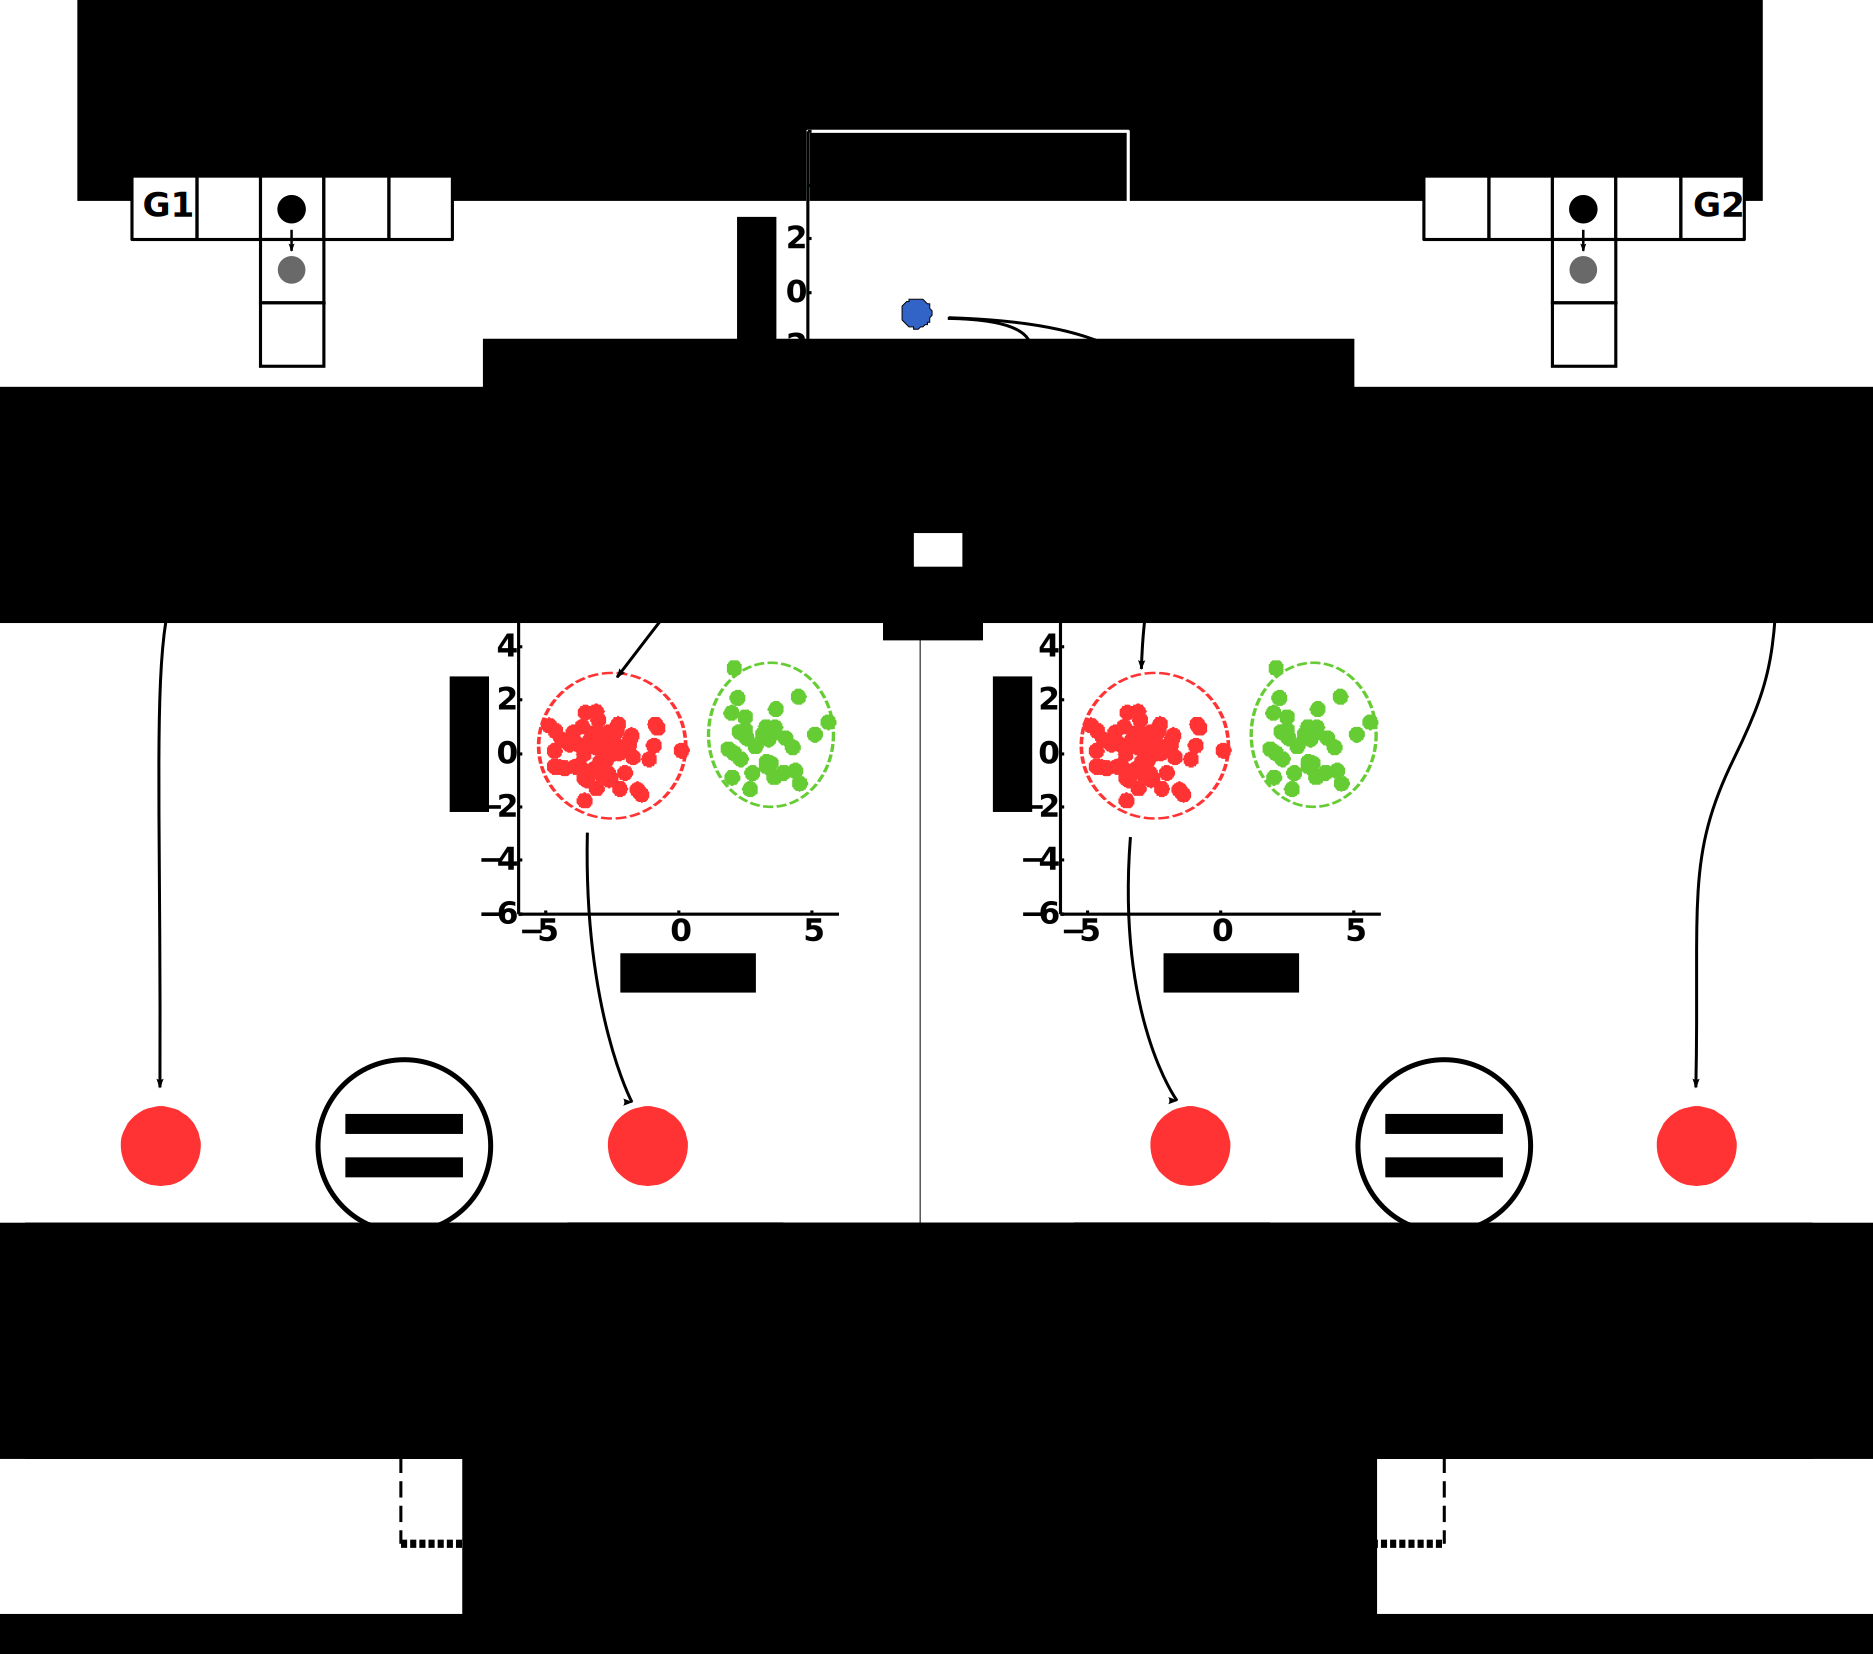
\includegraphics[width=\threeplanningwidth\columnwidth]{\visualspdf/planning/planning_up_down_expected_matched.pdf}
  \caption{Matching between expected labels and the prediction of a teaching signal sample on the left side of the feature space for the two hypothesis if the agent performs action down in state 3 and the two hypothesis currently have a symmetric interpretation of signals from Figure~\ref{fig:planningupdown}. Both hypothesis agree that the label associated to a signal on the left side of the feature space match with the label predicted given the frame and the state-action pair considered. Therefore there is no uncertainty associated to this state-action pair and the agent should not select action down in order to disambiguate between hypothesis.}
  \label{fig:uncertaintymeaningupdownexpectedleft}
\end{figure}

However for action left, the two hypothesis disagree on whether such signals are expected or not given the state-action pair considered. As depicted in Figure~\ref{fig:uncertaintymeaningupdownunexpectedright}, when selecting action left in state 3 and if the user sends a signal in the right part of the feature space, hypothesis 1 expects a signal of meaning ``correct'', and the teacher signal is classified as being of class ``correct''. And hypothesis 2 expects a signal of meaning ``incorrect'' and the teacher signal is classified as being of class ``correct''. Therefore receiving this particular signal after taking action down in state 3 is expected for hypothesis 1 but not expected for hypothesis 2, there is high uncertainty.

\begin{figure}[!ht]
  \centering
  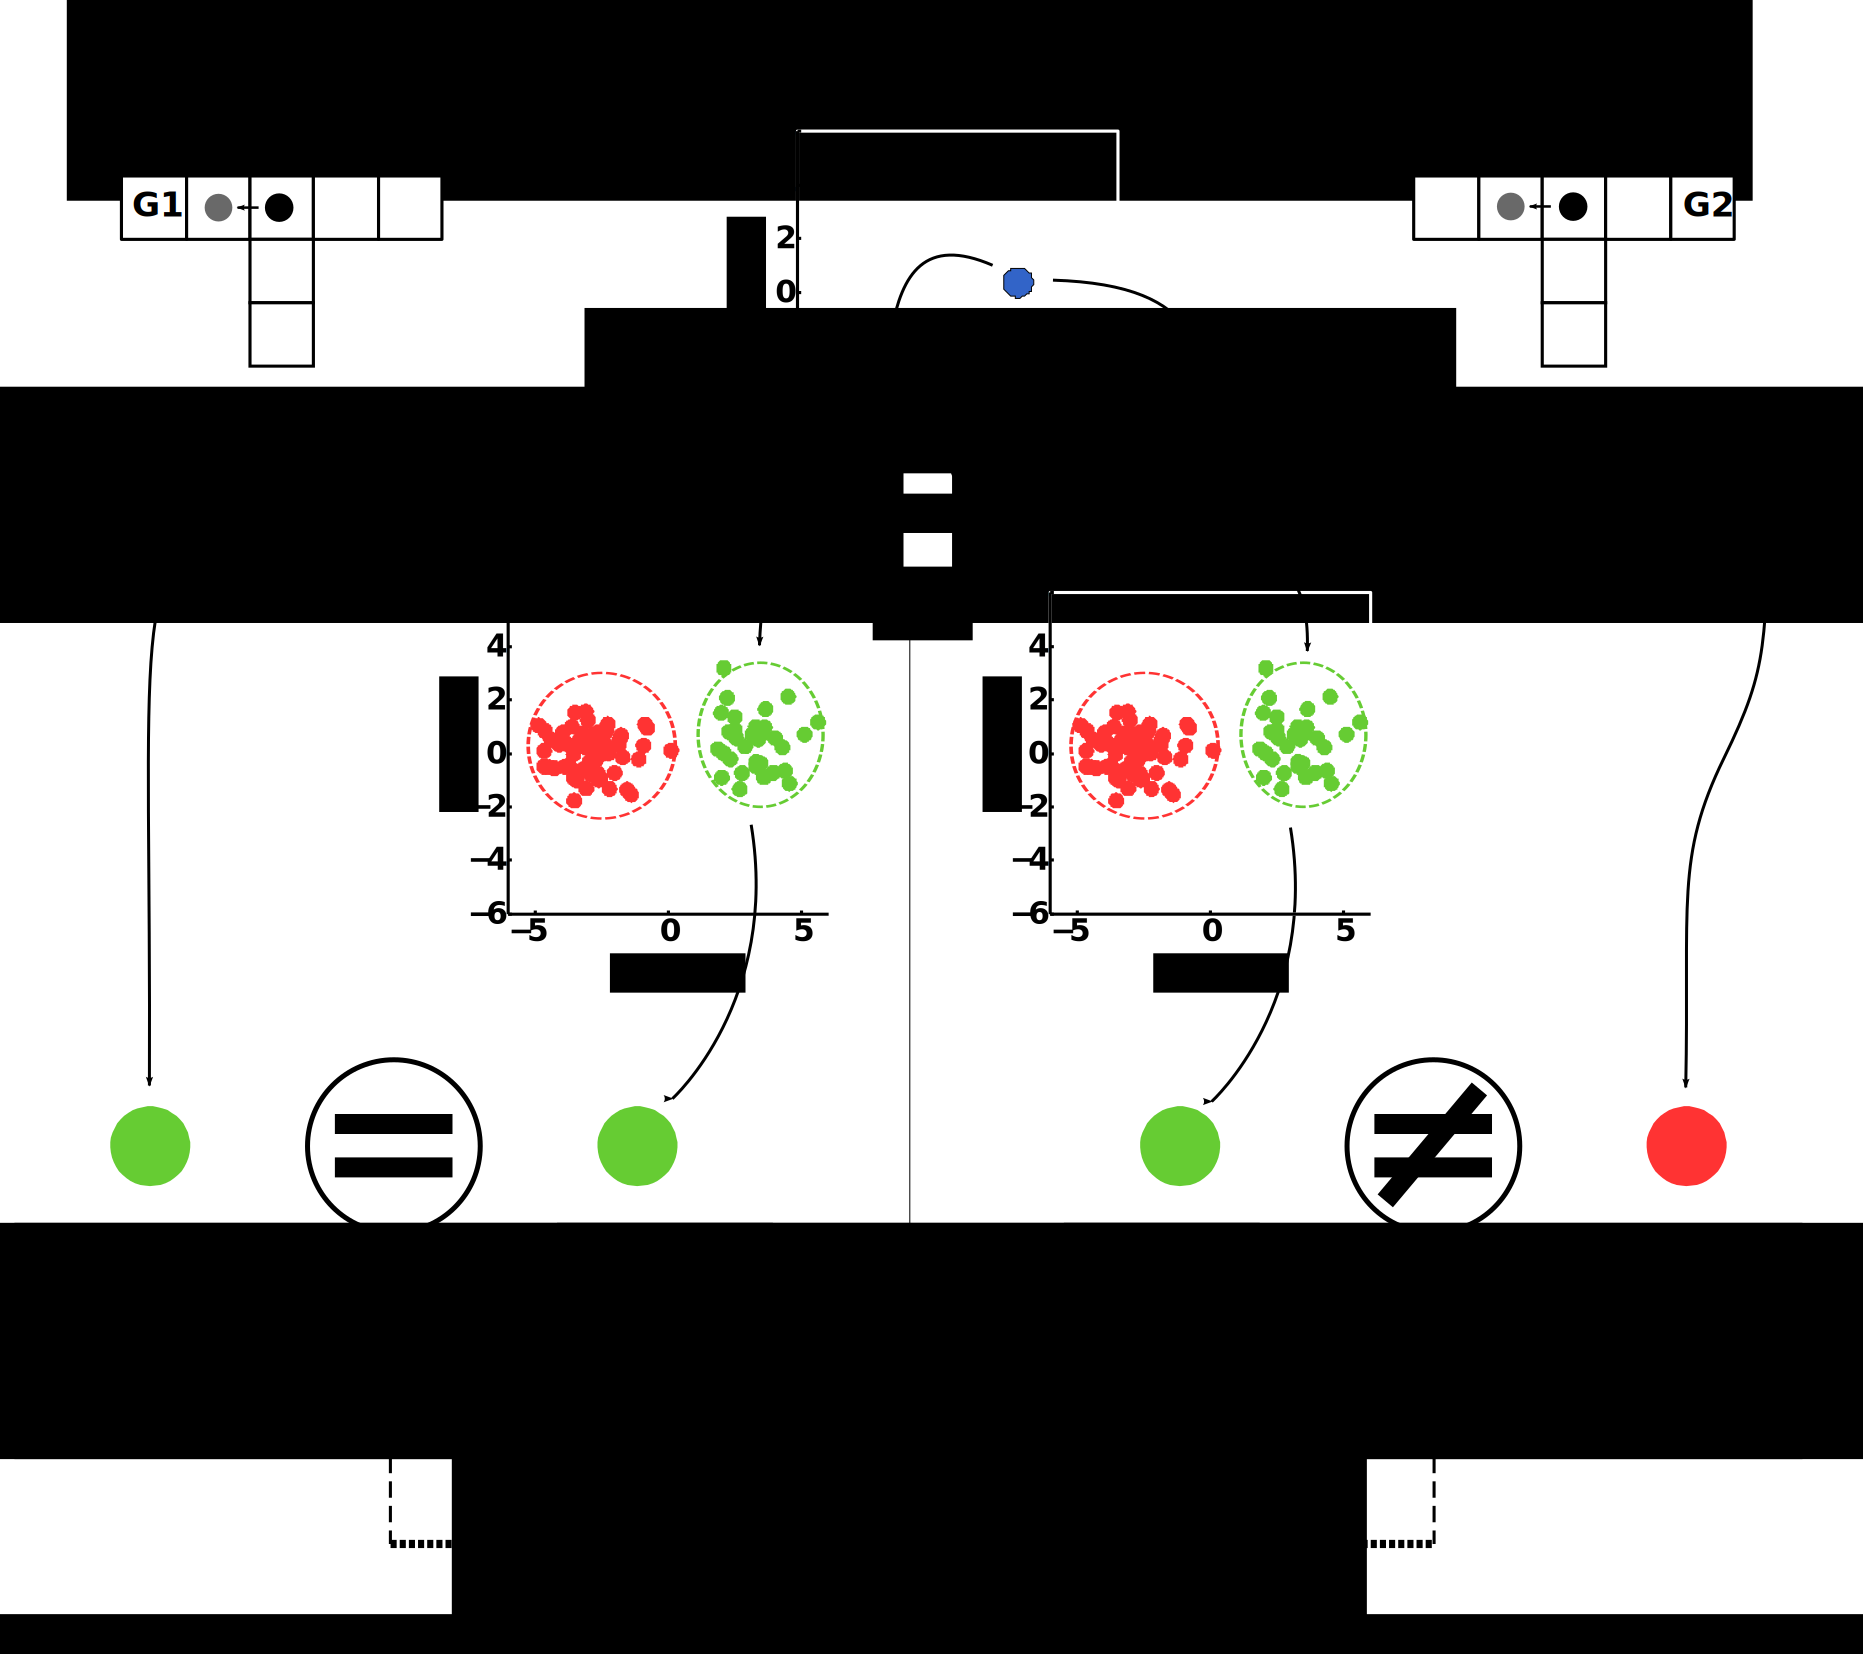
\includegraphics[width=\threeplanningwidth\columnwidth]{\visualspdf/planning/planning_up_down_unexpected_right_signal.pdf}
  \caption{Matching between expected labels and the prediction of a teaching signal sample on the right side of the feature space for the two hypothesis if the agent performs action left in state 3 and the two hypothesis currently have a symmetric interpretation of signals from Figure~\ref{fig:planningupdown}. Hypothesis 1 says a signal on the right side of the feature space means ``correct'' which was expected given the interaction frame, while hypothesis 2 expected a signal meaning ``incorrect'' but classify the signal as ``correct'' which was not expected. Therefore there is high uncertainty associated to this state-action pair and the agent should better perform action left in order to disambiguate between hypothesis.}
  \label{fig:uncertaintymeaningupdownunexpectedright}
\end{figure}

Similarly, as depicted in Figure~\ref{fig:uncertaintymeaningupdownunexpectedleft}, considering a teaching signal on the left side of the feature space, if the agent performs action left in state 3, hypothesis 1 expects a signal of meaning ``incorrect'', and the teacher signal is classified as being of class ``incorrect''. And hypothesis 2 expects a signal of meaning ``incorrect'' and the teacher signal is classified as being of class ``correct''. Therefore receiving this particular signal after taking action down in state 3 is not expected for hypothesis 1 but expected for hypothesis 2, there is high uncertainty.

\begin{figure}[!ht]
  \centering
  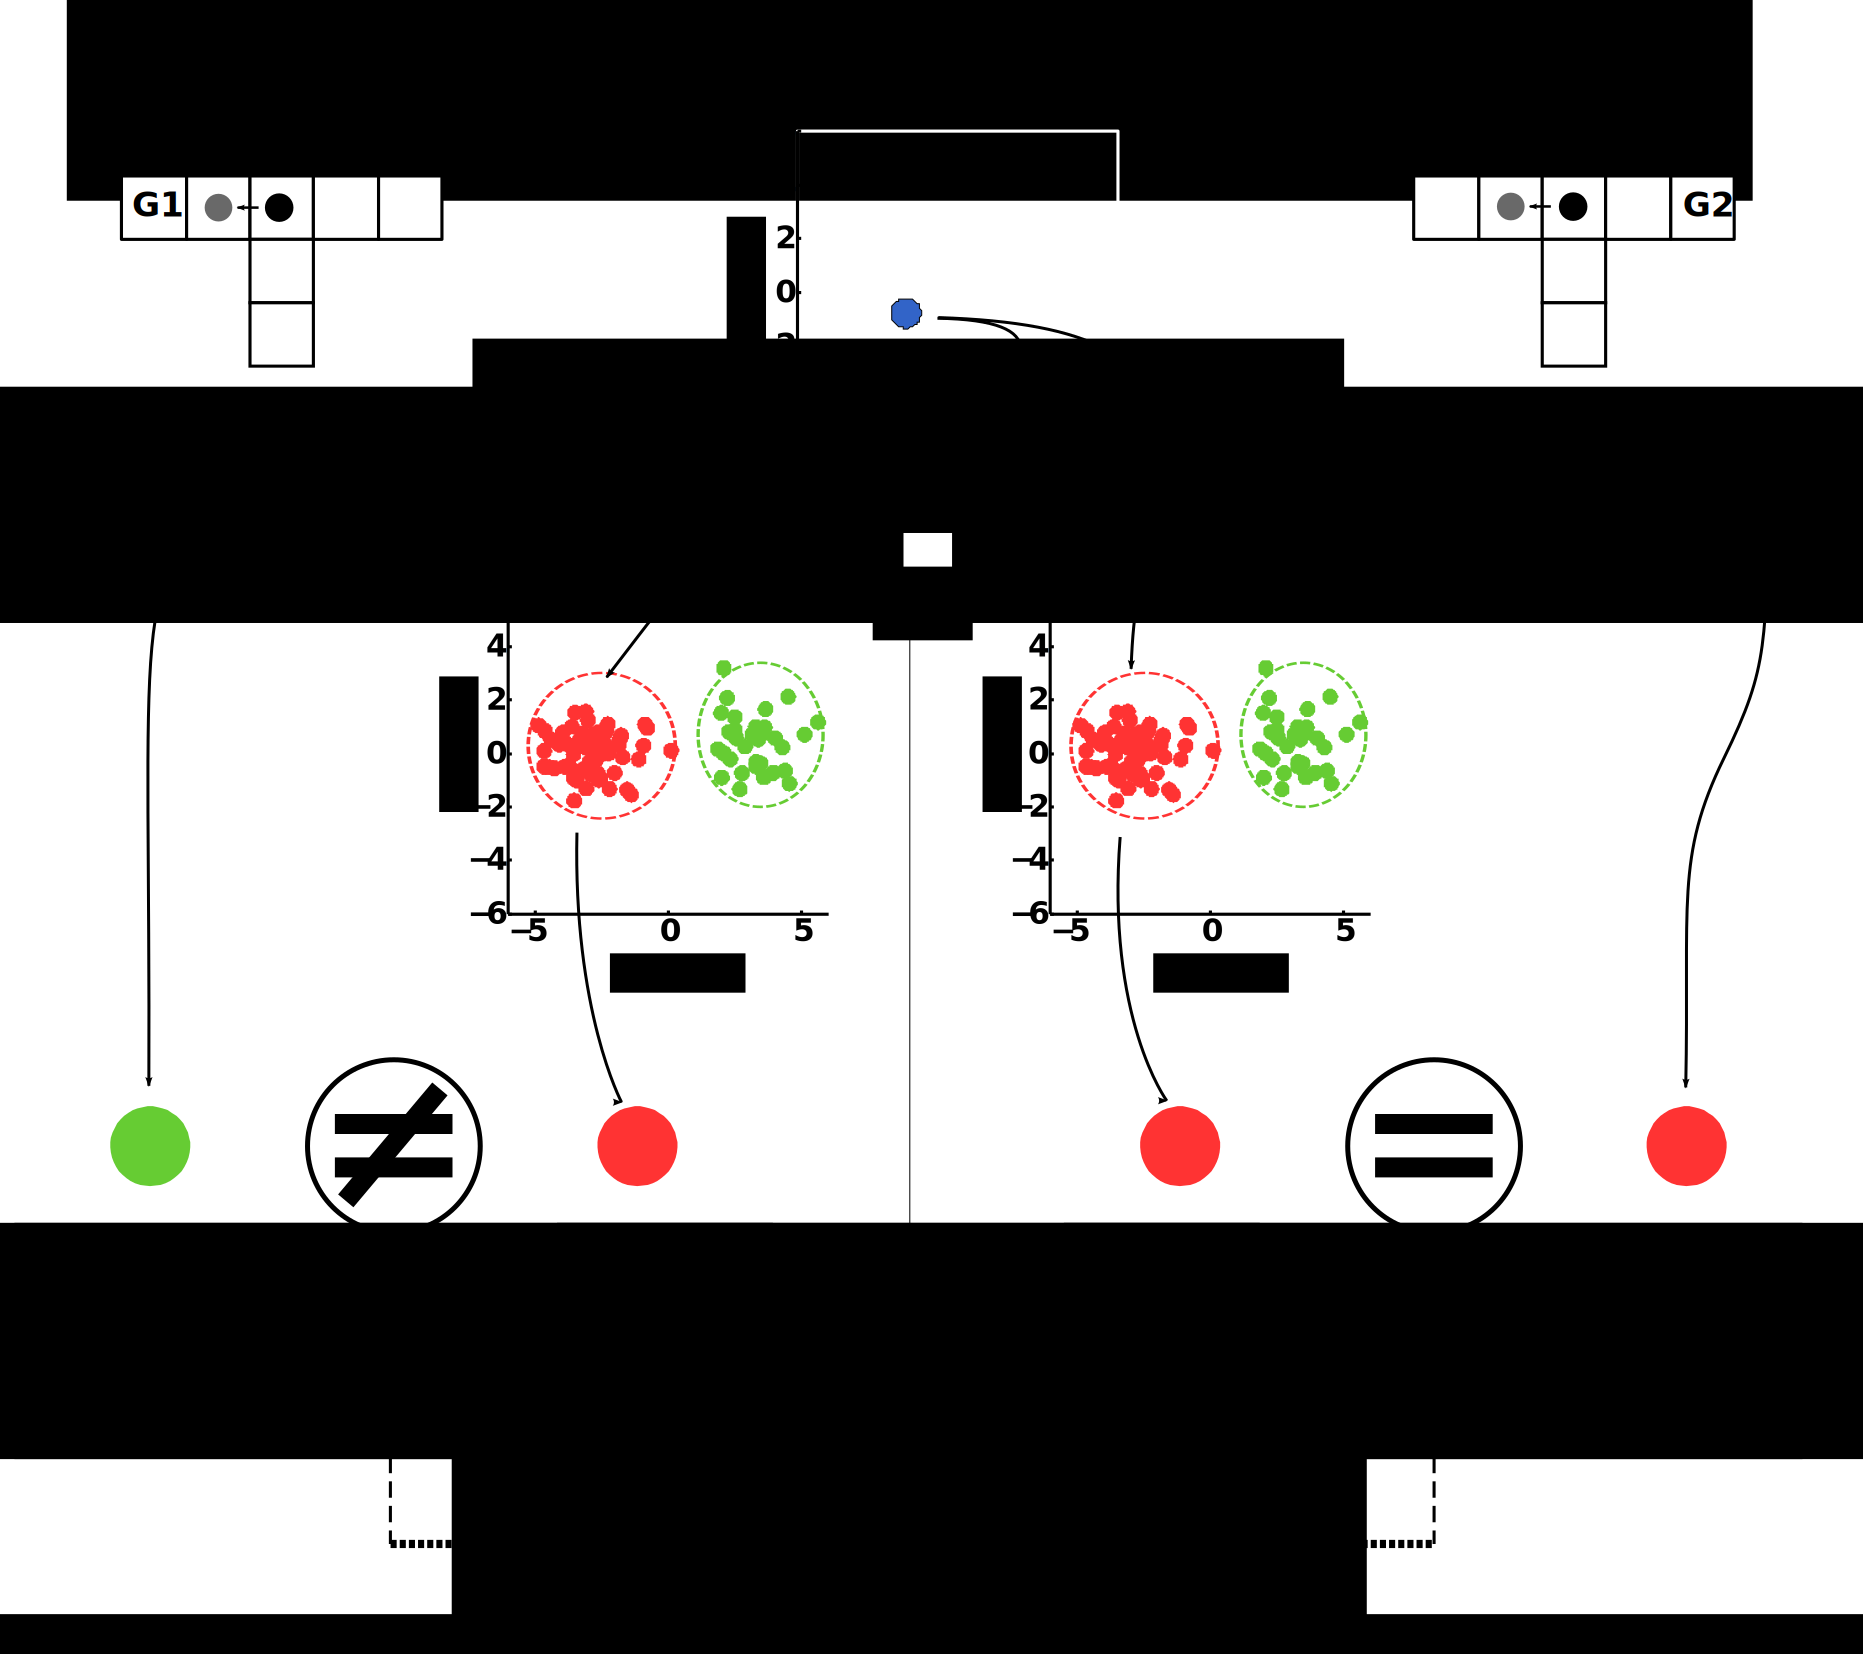
\includegraphics[width=\threeplanningwidth\columnwidth]{\visualspdf/planning/planning_up_down_unexpected_left_signal.pdf}
  \caption{Matching between expected labels and the prediction of a teaching signal sample on the left side of the feature space for the two hypothesis if the agent performs action left in state 3 and the two hypothesis currently have a symmetric interpretation of signals from Figure~\ref{fig:planningupdown}. Hypothesis 1 says a signal on the left side of the feature space means ``incorrect'' which was not expected given the interaction frame, while hypothesis 2 expected a signal meaning ``incorrect'' and classify the signal as ``incorrect'' which is what was expected. Therefore there is high uncertainty associated to this state-action pair and the agent should better perform action left in order to disambiguate between hypothesis.}
  \label{fig:uncertaintymeaningupdownunexpectedleft}
\end{figure}















